\documentclass[11pt]{article}
\title{Chain FPGA IP Catalog}
\date{August 15, 2019}
\author{Justen G. Di Ruscio}

\usepackage{amsmath}     % math formatting
\usepackage{graphicx}    % inserting figures
\usepackage{subcaption}  % subfigures
\usepackage{booktabs}    % top/bottom/midrule
\usepackage{multirow}    % wide table rows&cols
\usepackage{float}       % strict in place float position
\usepackage{caption}     % remove certain tables from list

\setcounter{tocdepth}{2}
	
\begin{document}
\pagenumbering{gobble}                                  % no numbers on title	
\maketitle
\begin{abstract}
	This document contains operational descriptions for the intellectual property created by Justen Di Ruscio in the Summer of 2019 for use in Jay-1
	ionosonde. However, this document is not a complete list of Justen's tasks during this time. All intellectual property listed is packaged hardware
	defining code, Verilog or SystemVerilog, to be implemented on a field programmable gate array. The designs illustrated are components of the Jay-1 
	ionosonde created by the Canadian High Arctic Ionospheric Network.
\end{abstract}
\section*{Relevant Information}
	Throughout this catalog, \textit{IP} will be used as the acronym for \textit{intellectual property}, and \textit{IF} will refer to 
	\textit{interface}. In addition, \textit{FPGA} describes a \textit{field programmable gate array}, \textit{BRAM} stands for 
	\textit{Block Random Access Memory}, and \textit{AXI} refers to the \textit{Advanced eXtensible Interface}, of which, AXI-Lite and AXI-Stream are 
	used. For all listed IP, at least one test bench and post-synthesis test has been completed. Vivado was the development tool used for all components
	,and the Genesys2 development board, using a Kintex-7 FPGA, is the target device.
\newpage
\pagenumbering{arabic}
\tableofcontents
\listoftables
\newpage

\section{Signal Paths}
To depict the purpose and use of the IP within the Jay-1 design, the input and output signal paths are shown below. It's important to understand
the purpose and use of the blocks interfacing with the FPGA, which will be described in this document, but not the exact specifications of each block.
\subsection{Input Signal Path}
This is the path a received signal must travel, for a single input channel.
\begin{figure}[h!]
	\label{inSigPath}
	\centering
	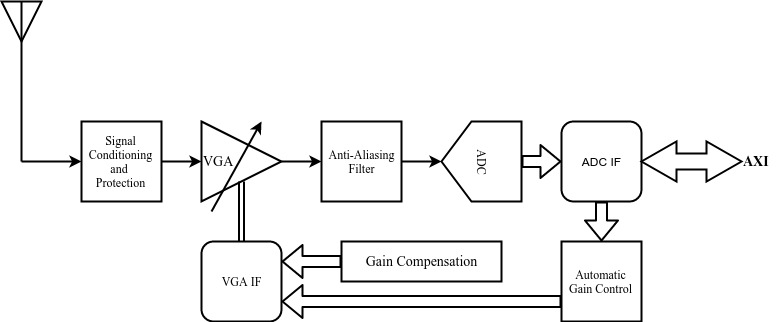
\includegraphics[width=0.8\linewidth]{images/inputSignalDiagram}
	\caption{Input Signal Path Block Diagram}
\end{figure}	
Of the above blocks, the VGA IF and ADC IF blocks, and all their contained IP, are components within this document.
\subsection{Output Signal Path}
This is the path a transmitted signal must travel, for a single output channel.
\begin{figure}[h!]
	\label{outSigPath}
	\centering
	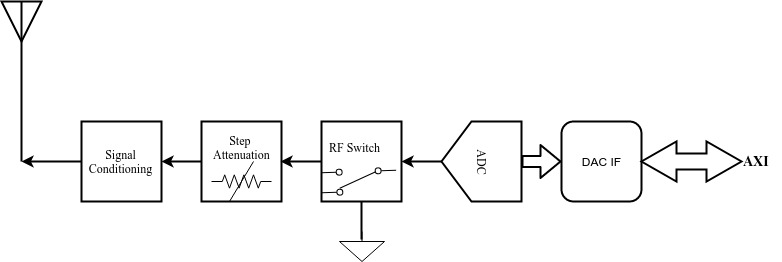
\includegraphics[width=0.8\linewidth]{images/outputSignalDiagram}
	\caption{Output Signal Path Block Diagram}
\end{figure}
Of the above blocks, the DAC IF, and all its contained IP, are components within this document.

\section{power\textunderscore meter}
Although the Power Meter was specifically created to measure the input power of of the ADC, located within the ADC IF, it is flexible and parameterized,
allowing it to measure any binary value. As as result, it is also implemented in the DAC\_ IF. Measurements by the power\textunderscore meter are 
done with respect to full scale input range, causing the measurements to actually report signal magnitude, but this extends to signal power measurements
based on the signal termination used.
\subsection{Diagram}
\begin{figure}[h!]
	\label{fig:powerMeter}
	\centering
	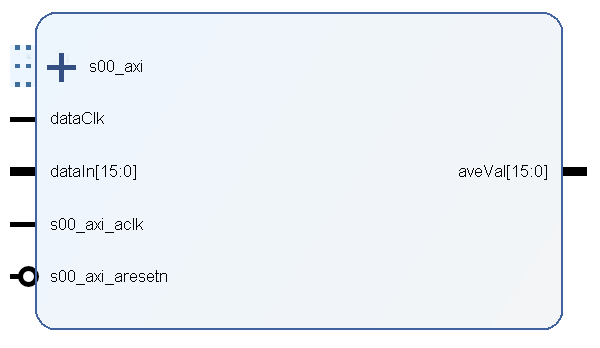
\includegraphics[width=0.6\linewidth]{images/powerMeter}
	\caption{IP Integrator Diagram of the power\textunderscore meter}
\end{figure}
\subsection{Parameters}
Non-AXI related parameters:
\begin{description}
	\item[sampleSize]Number of bits composing samples. Scales the channel size of dataIn and aveVal. Should be between 1-16bits for current design.
\end{description}
\subsection{Pin Description:}
\begin{description}
	\item[dataIn]Parallel input channel for data
	\item[dataClk]Clock used to govern rate at which data is sampled from dataIn
	\item[aveVal]Parallel output channel containing the sample average over the specified integration window
	\item[s00\textunderscore{}axi\textunderscore{}aclk]Positive edge sensitive clock governing data rate of AXI-Lite interface
	\item[s00\textunderscore{}axi\textunderscore{}aresetn]Active low, asynchronous reset for AXI-Lite interface and power\textunderscore meter logic
	\item[s00\textunderscore{}axi]Channel containing pins for the AXI-Lite specification. This IP acts as a slave
\end{description}
\subsection{AXI Register Mapping}
\begin{table}[h!]
	\centering
	\caption{power\textunderscore meter AXI-Lite Register Map}
	\label{powerMeterRegMap}
	\begin{tabular}{p{1.5cm}|p{1.5cm}|c|c|c|c|c|c}
		\toprule
		\textbf{Register Name}&\textbf{Address Offset}&\multicolumn{6}{c}{\textbf{Register Map (32bits per reg.)}}\\
		\midrule
		% slv_reg0
		\multirow{2}{*}{slv\textunderscore{}reg0}&\multirow{2}{*}{4'h0}&\multicolumn{2}{c|}{Unused}&\multicolumn{2}{c|}{Trigger}&
			\multicolumn{2}{c}{integrationWindowPower}\\
		\cline{3-8}
		&&\multicolumn{2}{c|}{bits 31-5}&\multicolumn{2}{c|}{bit 4}&\multicolumn{2}{c}{bits 3-0}\\
		\hline
		% slv_reg1
		\multirow{2}{*}{slv\textunderscore{}reg1}&\multirow{2}{*}{4'h4}&\multicolumn{4}{c|}{Unused}&\multicolumn{2}{|c}{calcDone}\\
		\cline{3-8}
		&&\multicolumn{4}{c|}{bits 31-1}&\multicolumn{2}{|c}{bit 0}\\
		\hline		
		% slv_reg2
		\multirow{2}{*}{slv\textunderscore{}reg2}&\multirow{2}{*}{4'h8}&\multicolumn{4}{c|}{peakADCVal}&\multicolumn{2}{c}{aveADCVal}\\
		\cline{3-8}
		&&\multicolumn{4}{c|}{bits 31-16}&\multicolumn{2}{c}{bits 15-0}\\
		\hline		
		% slv_reg3
		\multirow{2}{*}{slv\textunderscore{}reg3}&\multirow{2}{*}{4'hC}&\multicolumn{6}{c}{Unused}\\
		\cline{3-8}
		&&\multicolumn{6}{c}{bits 31-0}\\
		\bottomrule
	\end{tabular}	
\end{table}
\subsection{AXI Register Description}
\begin{description}
	\item[trigger (w)]Active high flag to start the sampling cycle of the power\textunderscore meter
	\item[integrationWindowPower (w)]Specifies the size of the integration window as $2^{integrationWindowPower}$
	\item[calcDone (r)]Active high flag indicating when the power\textunderscore meter has completed its calculations
	\item[peakADCVal (r)]Largest sample recorded on dataIn over integration window
	\item[aveADCVal (r)]Average sample value over the integration window
\end{description}
\subsection{Usage}
A reset pulse should be delivered at boot up to initialize all registers in the device. Once reset is complete, the device will wait for the trigger bit
to be asserted, where the power\_meter will read the integration window power from the respective AXI register to calculate the integration window size.
A valid trigger is a positive edge of the trigger bit while the device is not currently sampling data, indicated by the calcDone flag. Only at a valid 
trigger will the integration window power be sampled; however, both registers can be written to at any time. This property is useful for clearing the
trigger bit while the Power Meter is busy.\hfill\break
On dataClk rising edges following a valid trigger, the calcDone bit will be asserted low and the Power Meter
will sample the dataIn channel. After the integration window number of samples have been acquired, the calcDone flag will be asserted high, and
the average and peak sample will be written to their respective AXI register and average output pins. At this point, the power meter can repeat its
operation cycle. 

\section{IDELAYBUFDS}
The IDELAYBUFDS contains a configurable number of IDELAYE2 and IBUFDS Xilinx primitive pairs. Information regarding these internal primitives can be found
in the \textit{UG953} reference guide, also by Xilinx. In this IP, the IDELAYE2 is used in fixed delay mode, placed after the IBUFDS.
\subsection{Diagram}
\begin{figure} [h!]
	\label{fig:IDELAYBUFDS}
	\centering
	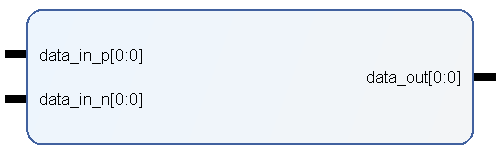
\includegraphics[width=0.6\linewidth]{images/IDELAYBUFDS}
	\caption{IP Integrator Diagram of the IDELAYBUFDS}	
\end{figure}
\subsection{Parameters}
\begin{description}
	\item[ioStandard]String describing the I/O standard used in the IBUFDS. The default option is ``LVDS\textunderscore25", but other options can be found
		in DS182 - the Kintex-7 datasheet linked below
	\item[dataWidth]Number of IDELAYE2/IBUFDS combination channels to create in IP
	\item[lowPower\textunderscore buf]Enables or disables low power mode of the IBUFDS in exchange for performance. Available options are ``TRUE" and
		``FALSE"
	\item[highPerformance\textunderscore delay]Enables or disables high performance mode of the IDELAYE2 in exchange for power savings. Available options
		are ``TRUE" and ``FALSE"
	\item[refClkFreq]The frequency in MHz of the reference clock, provided through an IDELAYCTRL module. Available value are 190-210 MHz and 290-310 MHz
		for the 7-Series FPGAs
	\item[diffTermination]Enables or disables the input differential termination resistance between the input terminals. Available options are ``TRUE"
		and ``FALSE"
	\item[delayTapVal]Selectable tap value which selects the delay imposed upon the signal, equal to $1/(64\times refClkFreq)\mu{}S$, where refClkFreq is
		in MHz
	\item[signalType]Describes the signal type for the IDELAYE2. Available values are ``CLOCK" and ``DATA", and the default value is ``DATA". This 
		allows the timing analyzer to account for jitter in the delay-chain
\end{description}
\subsection{Pin Description}
\begin{description}
	\item[data\textunderscore in\textunderscore p]Positive input channal for all IBUFDS/IDELAYE2 pairs
	\item[data\textunderscore in\textunderscore n]Negative input channal for all IBUFDS/IDELAYE2 pairs
	\item[data\textunderscore out]Single ended output channel for all IBUFDS/IDELAYE2 pairs
\end{description}
\subsection{Usage}
As this IP includes an IDELAYE2, it requires an IDELAYCTRL device to be instantiated in the same design in order to maintain calibration. Although there
is not a physical wire routed between the two, there is an internal bus designated for the reference clock signals in the FPGA, and once both are
instantiated, they will be placed on this bus upon implementation.\hfill\break
Each line in the input or output channel corresponds to the input or output with the same address. For example data\_in\_p[2], data\_in\_n[2], and data
\_out[2] are the pins to the same IBUFDS/IDELAYE2 pair.\hfill\break
The inputs should be routed to physical input pins on the FPGA chip.

\section{custom\textunderscore IBUFDS}
The custom\textunderscore IBUFDS is simply an extensible wrapper around the IBUFDS primitive, from Xilinx. This not only allows multiple differential
channels within a single IP, but also extends the internal IBUFDS's functionality to cooperate with data signals instead of just clock signals. Further
information regarding the internal IBUFDS primitive from Xilinx can be found in the \textit{UG953} reference guide.
\subsection{Diagram}
\begin{figure} [h!]
	\label{fig:custom_IBUFDS}
	\centering
	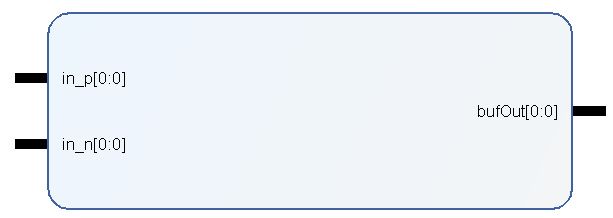
\includegraphics[width=0.6\linewidth]{images/custom_IBUFDS}
	\caption{IP Integrator Diagram of the custom\textunderscore IBUFDS}
\end{figure}
\subsection{Parameters}
\begin{description}
	\item[diffTerm]Enables or disables the input differential termination resistance between the inputs terminals. Available options are ``TRUE"
		and ``FALSE". The default is ``FALSE"
	\item[lowPower]Enables or disables low power mode of the IBUFDS in exchange for performance. Available options are ``TRUE" and ``FALSE". The default
		is ``FALSE"
	\item[ioStandard]String describing the I/O standard used in the IBUFDS. The default option is ``LVDS\textunderscore25", but other options can be found
		in DS182 - the Kintex-7 datasheet linked below
	\item[size]Number of differential channels to instantiate internally
\end{description}
\subsection{Pin Description}
\begin{description}
	\item[in\textunderscore p]Positive data inputs for all channels
	\item[in\textunderscore n]Negative data inputs for all channels
	\item[bufout]Single ended outputs for all channels
\end{description}
\subsection{Usage}
Compatible with data and clock signals. Ensure the I/O standard is set to meet the differential I/O standard driving the input lines.
The inputs should be routed to physical input pins on the FPGA chip.

\section{delay\textunderscore FIFO}
The delay\textunderscore FIFO is essentially a hardware BRAM asynchronous FIFO which prevents reading until the specified number of words have been
written. This delays the digital values by storing them internally.\hfill\break
The underlying FIFO is an xpm\textunderscore fifo\textunderscore async, which is a
macro provided by Xilinx that instantiates the necessary BRAM elements, based on the parameters specified. These BRAM elements will be connected together 
to meet the size requirement, up to 150 Mbits. Most of the tight timing restrictions and operating conditions inherent to BRAM devices, including the
xpm\textunderscore fifo\textunderscore async, are managed by the delay\textunderscore FIFO wrapper. Status flags are also available on this device which
fire under certain states, referred to as `protection pins', as they can protect the device from misuse. All protection pins are accessible
through the available AXI-Lite interface and are optionally enabled as discrete hardware lines. The IP is completely extensible and parameterized.
As such, it can be configured to fit most applications of varying requirements. Refer the \textit{UG953} reference guide for timing diagrams of the
Xilinx macro in specific situations.
\subsection{Diagrams}
\begin{figure}[H]
	\centering
	\begin{subfigure}[b]{0.4\linewidth}
		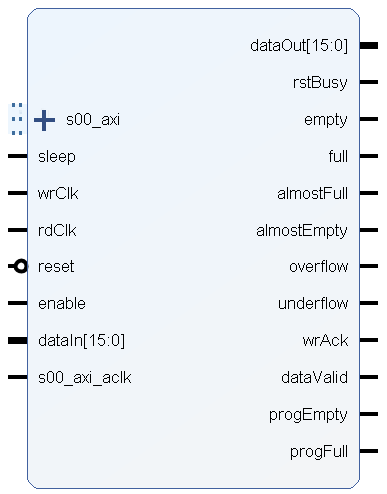
\includegraphics[width=\linewidth]{images/delay_FIFO}
		\caption{All Pins Enabled}
	\end{subfigure}
	\begin{subfigure}[b]{0.4\linewidth}
		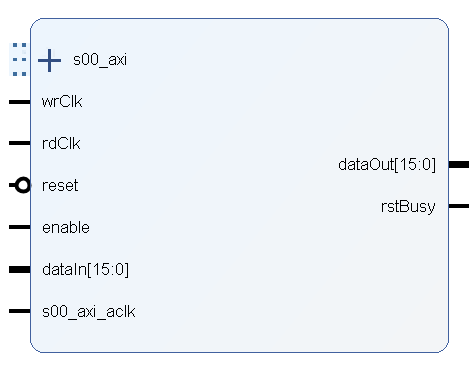
\includegraphics[width=\linewidth]{images/delay_FIFO_default}
		\caption{Default Settings}
	\end{subfigure}
	\caption{IP Integrator Diagram of the delay\textunderscore FIFO}
\end{figure}
\subsection{Parameters}
Non-AXI related parameters:
\begin{description}
	\item[fifoWidth]Width, from 1 to 4096, of FIFO. This scales input and output channel sizes and the number of instantiated BRAM elements
	\item[fifoDepth]Depth, from 16 to 4194304, of FIFO. This scales the maximum available delay value and number of instantiated BRAM elements
	\item[resetVal]Hexadecimal string representing the value on the output channel during reset. Default is ``0"
	\item[addrWidth]Number of bits used to address elements within BRAM. Automatically calculated and is not available in the graphical tool, but may be
		overriden in RTL if required 
	\item[readMode]Selects the read mode. Available options are ``std", which is the default, or ``fwft", which selects first word fall through operation.
	\item[rd\textunderscore clk\textunderscore delay \textunderscore en]Single bit used to enable the read clock for delay timing instead of the write
		clock, which is the default. Available options are 1'b0, the default, or 1'b1
	\item[prog\textunderscore full\textunderscore empty\textunderscore val]Number of words away from completely full or empty at which the
		prog\textunderscore full or prog\textunderscore empty flags are respectively asserted. Only used if
		prog\textunderscore full\textunderscore empty\textunderscore en is set to ``1".
	\item[advancedFeatures]Hexadecimal string representing a 13-bit word used to enable features of the hardware FIFO. The default value is ``1B1B" and 
		each bit within the word is active high. Locations of the features within the 13-bit configuration word is shown below:
		\begin{itemize}
			\item\textbf{bit 0} overflow flag
			\item\textbf{bit 1} prog\textunderscore full flag (programmable full)
			\item\textbf{bit 3} almost\textunderscore full flag
			\item\textbf{bit 4} wr\textunderscore ack flag (write acknowledge)
			\item\textbf{bit 8} underflow flag
			\item\textbf{bit 9} prog\textunderscore empty flag (programmable empty)
			\item\textbf{bit 11} almost\textunderscore empty flag
			\item\textbf{bit 12} data\textunderscore valid flag\\
			\textit{Note:} Unlisted bits are unused and should be set to 0.
		\end{itemize}
		As an example, if a user only wants the overflow flag enabled in hardware, they should set this parameter to ``1"
	\item[almost\textunderscore full\textunderscore empty\textunderscore en]Single bit enabling or disabling the external almostEmpty and almostFull pins
	\item[prog\textunderscore full\textunderscore empty\textunderscore en]Single bit enabling or disabling the external progEmpty and progFull pins
	\item[over\textunderscore under\textunderscore flow\textunderscore en]Single bit enabling or disabling the external underflow and overflow pins
	\item[wr\textunderscore ack\textunderscore en]Single bit enabling or disabling the external wrAck (write acknowledge) pin
	\item[data\textunderscore valid\textunderscore en]Single bit enabling or disabling the external dataValid pin
	\item[full\textunderscore empty\textunderscore en]Single bit enabling or disabling the external empty and full pins
	\item[sleep\textunderscore en]Single bit enabling or disabling the external sleep input pin
\end{description}
\subsection{Pin Description}
\begin{description}
	\item[sleep]When either this line, or the sleep bit in the AXI register, go high, the FIFO enters a dynamic power saving mode
	\item[wrClk]Write clock: rising edges of this line clock data into the FIFO. This is also the default delay timing clock when the 
		rd\textunderscore clk\textunderscore delay\textunderscore en parameter is set to 1'b1 
	\item[rdClk]Read clock: rising edges of this line clock data out of the FIFO once the specified number of words have been written into the FIFO as
		delay. This can also be used as the delay timing clock when the rd\textunderscore clk\textunderscore delay\textunderscore en parameter is set to
		1'b1
	\item[reset]Active low reset. A negative edge of this line, or the negative edge of the reset bit in the AXI register, will cause the
		FIFO to enters its reset sequence, indicated by the rstBusy line.
	\item[enable]Active high enable pin. When this pin, or the enable bit in the AXI register, go high, the FIFO is enabled, allowing writes and reads.
		However, the device will only be enabled when: the device is not currently in its reset sequence (indicated by the rstBusy line); both reset
		inputs are inactive; and when the disable bit in the AXI register is low. All of these take precedence over an asserted enable line
	\item[dataIn]Input channel for data. So long as the device is enabled, the value on these lines will be written into the FIFO upon a rising
		wrClk (write clock) edge
	\item[dataOut]Output channel for data. So long as the device is enabled, and the specified delay has been met, the eldest word written into the FIFO
		will be extracted and written to these lines.
	\item[rstBusy]Reset busy: internally asserted high while the device is within its reset sequence
	\item[empty]Asserted high when the FIFO is empty. A read from the FIFO while its empty will be ignored and is not destructive. This pin can be removed
		from the package using the full\textunderscore empty\textunderscore en parameter. Set until read flag
	\item[full]Asserted high when the FIFO is full. A write to the FIFO while its full will be ignored and is not destructive. This pin can be removed
		from the package using the full\textunderscore empty\textunderscore en parameter. Set until read flag
	\item[almostFull]Asserted high when the FIFO is one word away from being full. This pin can be removed from the package using the
		almost\textunderscore full\textunderscore empty\textunderscore en parameter. Set until read flag
	\item[almostEmpty]Asserted high when the FIFO is one word away from being empty (contains only a single word). This pin can be removed from the
		package using the almost\textunderscore full\textunderscore empty\textunderscore en parameter. Set until read flag
	\item[overflow]Asserted high on the following wrClk edge after the FIFO becomes full and the device is enabled. The overflow will be ignored and will
		not be destructive. This pin can be removed from the package using the over\textunderscore under\textunderscore flow\textunderscore en parameter.
		Set until read flag
	\item[underflow]Asserted high on the following rdClk edge after the FIFO becomes empty and the device is enabled. The underflow will be ignored and
		will not be destructive. This pin can be removed from the package using the over\textunderscore under\textunderscore flow\textunderscore en
		parameter. Set until read flag
	\item[wrAck]Write acknowledge: set high for a clock cycle indicating the write to the FIFO on the previous write clock edge was accepted. This pin can
		be removed from the package using the wr\textunderscore ack\textunderscore en parameter. Set until read flag
	\item[dataValid]Flag asserted high while there is valid data on the output port, and low otherwise. This pin can be removed from the package using the
		data\textunderscore valid\textunderscore en parameter. Set until read flag
	\item[progEmpty]Programmable empty: flag set high when FIFO reaches programmable empty threshold. This pin can be removed from the package using the
		prog\textunderscore full\textunderscore empty\textunderscore en parameter. Set until read flag
	\item[progFull]Programmable full: flag set high when FIFO reaches programmable full threshold. This pin can be removed from the package using the
		prog\textunderscore full\textunderscore empty\textunderscore en parameter. Set until read flag
	\item[s00\textunderscore axi]Bus containing pins for AXI-Lite specification. This IP acts as a slave
\end{description}
\subsection{AXI Register Mapping}
\begin{table}[H]
	\centering
	\caption{delay\textunderscore FIFO AXI Register Map}	
	\label{delayFIFORegMap_start}
	\begin{tabular}{p{1.5cm}|p{1.5cm}|c|c|c|c|c|c|p{0.5cm}}
		\toprule
		\textbf{Register Name}&\textbf{Address Offset}&\multicolumn{7}{c}{\textbf{Register Map (32bits per reg.)}}\\
		\midrule
		% slv_reg0
		\multirow{2}{*}{slv\textunderscore{}reg0}&\multirow{2}{*}{4'h0}&\multicolumn{6}{c|}{Unused}&...\\
		\cline{3-9}
		&&\multicolumn{6}{c|}{bits 31-26}&...\\
		\hline
		% slv_reg1
		\multirow{2}{*}{slv\textunderscore{}reg1}&\multirow{2}{*}{4'h4}&wrAck&dataValid&overflow&full&almostFull&progFull&...\\
		\cline{3-9}
		&&bit 31&bit 30&bit 29&bit 28&bit 27&bit 26&...\\
		\hline		
		% slv_reg2
		\multirow{2}{*}{slv\textunderscore{}reg2}&\multirow{2}{*}{4'h8}&\multicolumn{6}{c|}{Unused}&...\\
		\cline{3-9}
		&&\multicolumn{6}{c|}{bits 31-2}&...\\
		\hline		
		% slv_reg3
		\multirow{2}{*}{slv\textunderscore{}reg3}&\multirow{2}{*}{4'hC}&\multicolumn{6}{c|}{Unused}&...\\
		\cline{3-9}
		&&\multicolumn{6}{c|}{bits 31-0}&...\\
		\bottomrule
	\end{tabular}
	\hfill\break
	\begin{center}
	Table 2 Continued
	\end{center}
	\begin{tabular}{p{0.5cm}|c|c|c|c|c|c|c|}
		\toprule
		&\multicolumn{7}{c|}{\textbf{Register Map (32bits per reg.)}}\\
		\midrule
		% slv_reg0
		\multirow{2}{*}{...}&disable&sleep&reset&enable&\multicolumn{3}{c|}{delayValue}\\
		\cline{2-8}
		&bit 25&bit 24&bit 23&bit 22&\multicolumn{3}{|c|}{bits 21-0}\\
		\hline
		% slv_reg1
		\multirow{2}{*}{...}&progEmpty&almostEmpty&empty&underflow&\multicolumn{3}{|c|}{fifoDepth}\\
		\cline{2-8}
		&bit 25&bit 24&bit 23&bit 22&\multicolumn{3}{c|}{bits 21-0}\\
		\hline		
		% slv_reg2
		\multirow{2}{*}{...}&\multicolumn{4}{c}{Unused}&rstBusy&wrRstBusy&rdRstBusy\\
		\cline{2-8}
		&\multicolumn{4}{c|}{bits 31-2}&bit 2&bit 1&bit 0\\
		\hline		
		% slv_reg3
		\multirow{2}{*}{...}&\multicolumn{7}{c|}{Unused}\\
		\cline{2-8}
		&\multicolumn{7}{c|}{bits 31-0}\\
		\bottomrule
	\end{tabular}
\end{table}
\subsection{AXI Register Description}
\begin{description}
	\item[disable (w)]Overrides both of the enable inputs to disable the device. While disabled, both reads and writes are prevented
	\item[sleep (w)]When either this register, or the dedicated sleep line, go high, the FIFO enters a dynamic power saving mode
	\item[reset (w)]Active low reset. A negative edge of this register, or the negative edge of dedicated hardware line, will cause the
		FIFO to enters its reset sequence, indicated by the rstBusy line.
	\item[enable(w)]Active high enable register. When this register, or the dedicated hardware line, go high, the FIFO is enabled, allowing writes and
		reads. However, the device will only be enabled when: the device is not currently in its reset sequence (indicated by the rstBusy line); when both
		reset inputs are inactive; and when the disable bit in the AXI register is low. All of these take precedence over an asserted enable line
	\item[delayValue (w)]Sets the delayValue, the number of timer clock edges, chosen as the read clock or the write clock, to delay data through FIFO.
		This value can be set between three up to the fifoDepth; however, values above or below these thresholds will result in the limits being used, 
		preventing any harm. At reset, three is written to this register, allowing operation with the minimum delay without having to first
		having to write to any AXI register. Moreover, delayValue can be modified at runtime, but it should be noted that increasing and decreasing the
		delayValue at runtime each have their own operation
	\item[wrAck (r)]Write acknowledge: set high for a clock cycle indicating the write to the FIFO on the previous write clock edge was accepted.
		Set until read flag
	\item[dataValid (r)]Flag asserted high while there is valid data on the output port, and low otherwise. Set until read flag
	\item[overflow (r)]Asserted high on the following wrClk edge after the FIFO becomes full and the device is enabled. The overflow will be ignored and
		will not be destructive. Set until read flag
	\item[full (r)]Asserted high when the FIFO is full. A write to the FIFO while its full will be ignored and is not destructive. Set until read flag
	\item[almostFull (r)]Asserted high when the FIFO is one word away from being full. Set until read flag
	\item[progFull (r)]Programmable full: flag set high when FIFO reaches programmable full threshold. Set until read flag
	\item[progEmpty (r)]Programmable empty: flag set high when FIFO reaches programmable empty threshold. Set until read flag
	\item[almostEmpty (r)]Asserted high when the FIFO is one word away from being empty (contains only a single word). Set until read flag
	\item[empty (r)]Asserted high when the FIFO is empty. A read from the FIFO while its empty will be ignored and is not destructive. Set until read flag
	\item[underflow (r)]Asserted high on the following rdClk edge after the FIFO becomes empty and the device is enabled. The underflow will be ignored
		and will not be destructive. Set until read flag
	\item[fifoDepth (r)]Depth of the FIFO set in the parameter. Makes this available at runtime if needed
	\item[rstBusy (r)]Active high flag indicating that the FIFO is still in its reset sequence
	\item[wrRstBusy (r)]Active high flag indicating that the FIFO's write (input) port is specifically within a reset state in the overall reset sequence
	\item[rdRstBusy (r)]Active high flag indicating that the FIFO's read (input) port is specifically within a reset state in the overall reset sequence
\end{description}
\subsection{Usage}
This IP requires an initial reset pulse for proper operation. Once the rstBusy line indicates that the reset sequence has completed, the FIFO's enable
inputs become active; nevertheless, they can be driven to any state at any point without consequences. The FIFO can become enabled when either of the
enable lines are high, both of the reset lines are inactive (high), the FIFO is not currently in a reset procedure (indicated by the rstBusy line being
low), and the disable bit in the AXI register is low. Once enabled, the FIFO will start collecting samples at each rising wrClk edge.
After the specified number of timing clock edges, which can be either the rdClk or wrClk, reading from the FIFO will be permitted at every following
rdClk rising edge.\hfill\break
The delayValue bits within the AXI reg are used to select the number of timing clock edges used delay the input data. This delayValue can be three, the
default value, up to the fifoDepth specified as a parameter.
Changing the delayValue at runtime is permitted. Increasing the delayValue will cause the output data to remain fixed, and the dataValid flag to go low
until the larger delayValue has been met. So long as there is not an overflow, no input data will be lost during this procedure. Decreasing the delayValue
will cause the wrAck flag to be asserted low until the smaller delayValue has been met. To meet a smaller delay value, input samples must be ignored,
resulting in a small loss of data. Assuming a constant flow of input data, the samples following the write of the updated delayValue, to the samples
before the assertion of wrAck, are ignored. The difference between the current delayValue and the smalleer delayValue is the number of samples that get
ignored following a write of an updated delayValue.\hfill\break
At any point, the flags listed in Pin Description and  AXI Register Description will fire to indicate state and possibly protect the FIFO from application
specific errors. The flags which indicate they are \textit{set until read} flags will be set at their associated state but will only be cleared upon a
read of their respective register. These inform the user that the flag has been set since the last read of the register.\hfill\break
For optimal operation, the write clock and read clock should be of the same frequency with no preference of phase shift. This is not enforced, nor is it
required.

\section{adc\textunderscore IF\textunderscore core}
The adc\textunderscore IF\textunderscore core is an IP to specifically interface with the LTC2217 analog to digital converter within the input signal path
of the Jay-1 Ionosonde. It reads the 16-bit LVDS 2.5 V parallel data from the \textit{ADC}, acts as an AXI-Stream master to stream the samples to a slave,
and provides an AXI-Lite interface for configuration.\hfill\break
The input samples have two locations for delay tuning, one in the IDELAYBUFDS for phase matching with the clock, and another in the
delay\textunderscore FIFO for phase matching between adc\textunderscore IF\textunderscore core devices. The AXI-Stream data channel is generated by the
output of the delay\textunderscore FIFO. In addition, a power\textunderscore meter is contained within this IP to read the ADC power, directly after the
IDELAYBUFDS delay element. All AXI-Lite registers of the power\textunderscore meter and the delay\textunderscore FIFO are available through a single AXI-
Lite slave interface. Internally, this IP contains the logic to prevent data corruption from enablement or reset while the IP is busy, and logic to meet
reset requirements of contained IP.\hfill\break
Finally, the IP converts the LVDS overflow signal from the ADC to a single-ended signal for other IP to utilize. For further information on the LTC2217,
please refer to \textit{LT0108}.
\captionsetup[table]{list=no}   % exclude this from table list
\subsection{Contained IP}
\begin{table}[H]
	\centering
	\caption{Contained IP Within adc\textunderscore IF\textunderscore core}
	\begin{tabular}{p{6cm}|p{6cm}}
		\multicolumn{1}{c|}{\textbf{Custom IP}}&\multicolumn{1}{|c}{\textbf{Xilinx IP}}\\
		\toprule		
		\begin{itemize}
	 		\item custom\textunderscore channel\textunderscore IBUFDS
			\item power\textunderscore meter
			\item delay\textunderscore FIFO
			\item IDELAYBUFDS
		\end{itemize}
		&
		\begin{itemize}
			\item axi\textunderscore crossbar
			\item util\textunderscore reduced\textunderscore logic
			\item util\textunderscore vector\textunderscore logic
			\item xlconcat
			\item xlconstant
		\end{itemize}\\
	\end{tabular}
\end{table}
\captionsetup[table]{list=yes}   % include following tables
\subsection{Diagrams}
\begin{figure}[H]
	\centering
	\begin{subfigure}[b]{\linewidth}
		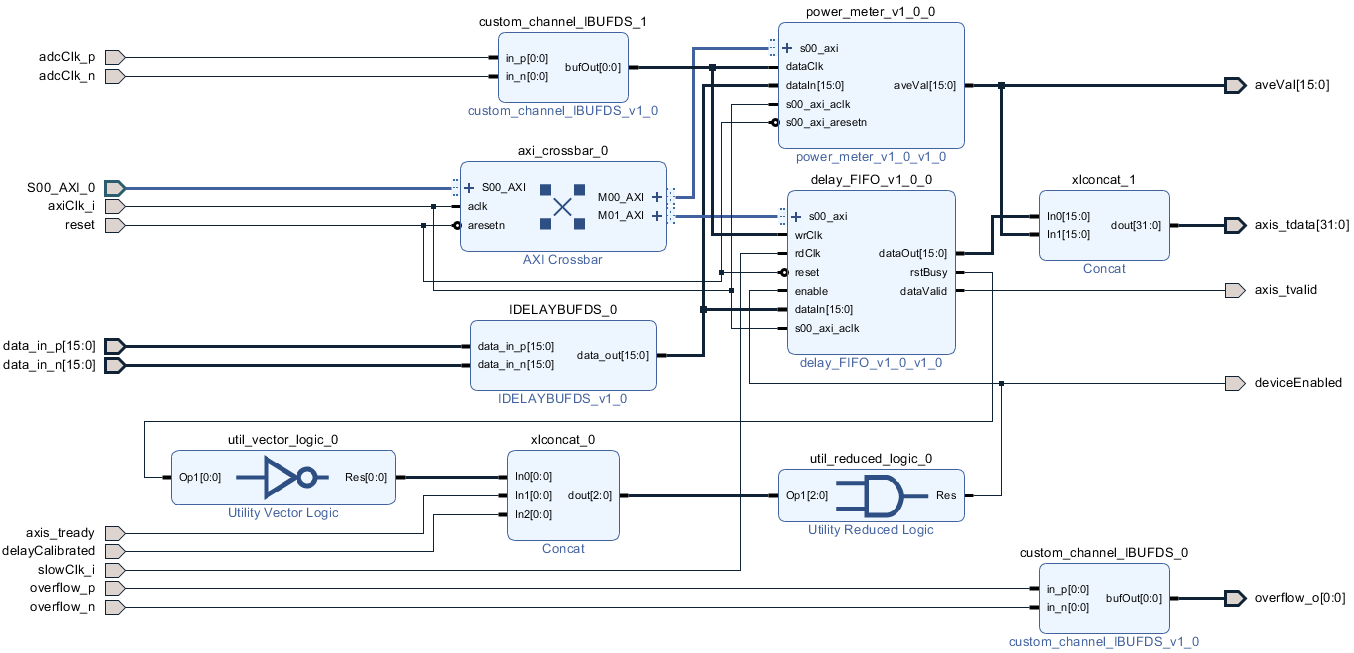
\includegraphics[width=\linewidth]{images/adc_IF_core_internal}
		\caption{Internal Diagram}
	\end{subfigure}
	\begin{subfigure}[b]{0.4\linewidth}
		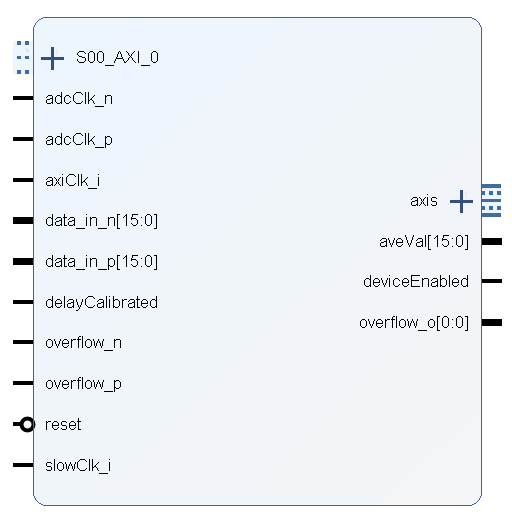
\includegraphics[width=\linewidth]{images/adc_IF_core}
		\caption{adc\textunderscore IF\textunderscore core Package}
	\end{subfigure}
	\caption{IP Integrator Diagrams of the adc\textunderscore IF\textunderscore core}
\end{figure}
\subsection{Parameters}
Since this IP is very specific to its application, it does not contain any global parameters. All internal IP is pre-configured to meet the application
requirements. Sadly, the IP flow does not support passing global parameters to internal IP, preventing externalizing composing IP's parameters. The 
delayTapVal parameter of the IDELAYBUFDS suffers most from this, as it may need modification to match the adcClk phase. If one would like to alter the
default parameters, they can do so by modifying the design in the IP Integrator and re-packaging.
\subsubsection{Internal IP Default Parameters}
Every IP has default parameters, most of which are obvious or are described by the IP operation. The important parameters are listed in the following
figures.
\begin{figure}[H]
	\centering
	\begin{subfigure}[t]{0.4\linewidth}
		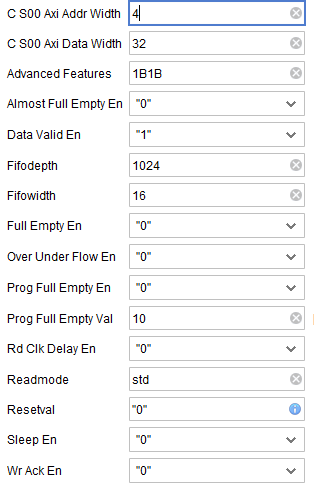
\includegraphics[width=\linewidth]{images/default_param_delay_FIFO}
		\caption{delay\textunderscore FIFO}
	\end{subfigure}
	\begin{subfigure}[t]{0.4\linewidth}
		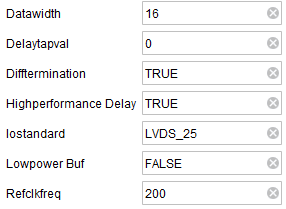
\includegraphics[width=\linewidth]{images/default_param_IDELAYBUFDS}
		\caption{IDELAYBUFDS}
	\end{subfigure}
	\begin{subfigure}[t]{0.4\linewidth}
		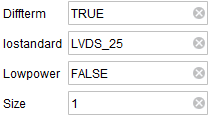
\includegraphics[width=\linewidth]{images/default_param_channel_IBUFDS}
		\caption{channel\textunderscore IBUFDS}
	\end{subfigure}
	\begin{subfigure}[t]{0.4\linewidth}
		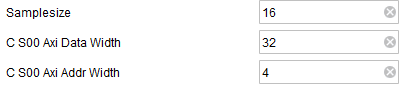
\includegraphics[width=\linewidth]{images/default_param_power_meter}
		\caption{power\textunderscore meter}
	\end{subfigure}
	\caption{Default Parameters of the adc\textunderscore IF\textunderscore core's Internal IP} 
	\label{fig:adcIFparams}
\end{figure}
\subsection{Pin Description}
\begin{description}
	\item[adcClk\textunderscore n]Negative input terminal for LVDS 2.5 V data rate clock from ADC
	\item[adcClk\textunderscore p]Positive input terminal for LVDS 2.5 V data rate clock from ADC
	\item[axiClk\textunderscore i]Single-ended input terminal for AXI-Lite
	\item[data\textunderscore in\textunderscore n]Negative input channel for LVDS 2.5 V data from ADC
	\item[data\textunderscore in\textunderscore p]Positive input channel for LVDS 2.5 V data from ADC
	\item[delayCalibrated]Flag from IDELAYCTRL module that must be instantiated within the same design as this IP. Informs the adc\textunderscore IF
		\textunderscore core that the delay filter is stable/calibrated. This IP is internally prohibited from reading or writing data to the AXI-Stream
		interface through the FIFO while this is low. The differential overflow buffer and power\textunderscore meter may still run while this line is
		low, but that is not recommended.
	\item[overflow\textunderscore n]Negative input terminal for LVDS 2.5 V overflow signal from LTC2217 ADC
	\item[overflow\textunderscore p]Positive input terminal for LVDS 2.5 V overflow signal from LTC2217 ADC
	\item[overflow\textunderscore o]Single-ended output terminal for overflow signal from LTC2217 ADC
	\item[slowClk\textunderscore i]Single ended input for internally generated `slow clock', which is a 105MHz clock that extracts data from the
		adc\textunderscore IF\textunderscore core through the AXI-Stream interface. This is essentially the AXI-Stream data clock and, as such, should
		be connected to the AXI-Stream input clock of the connected slave. The slow clock frequency should be that of the ADC sampling frequency, and
		should be connected to all adc\textunderscore IF\textunderscore cores, so they all extract data at the same time.
	\item[aveVal]16-bit, single-ended output channel from the internal power\textunderscore meter, relaying the average power for other hardware devices
	\item[reset]Active low reset for all device logic, including AXI-Lite interface
	\item[deviceEnabled]Status flag indicating the internal FIFO is enabled; this IP is able to receive samples. Specifically, this flag indicates:\hfill
		\begin{enumerate}
			\item delayCalibrated is high 
			\item AXI-Stream interface is ready, indicated by a logic 1 on the ready pin
			\item the FIFO is not within its reset procedure
			\item active low reset line is deactivated
		\end{enumerate}
	\item[axis]AXI-Stream interface. Contains necessary lines to match protocol. As these lines are simple enough to be implemented in a design with
		discrete logic, their purposes are listed below:\hfill
		\begin{description}
			\item[$\bullet$ axis\textunderscore tvalid]Indicates to the slave that valid data is available
			\item[$\bullet$ axis\textunderscore tready]Indicates to the master that the slave is ready for data
			\item[$\bullet$ axis\textunderscore tdata]32-bit data channel
		\end{description}
		A slave must only implement the axis\textunderscore tready signal and read the valid and data lines.
	\item[S00\textunderscore AXI\textunderscore 0]AXI-Lite bus containing all necessary lines for the protocol
\end{description}
\subsection{AXI Interface Mapping}
Both the AXI-Stream data channel mapping and the AXI-Lite address mapping are included in this section. For a detailed mapping of each register, please 
refer to the respective IP description above.
\subsubsection{AXI-Stream Interface}
\begin{table}[H]
	\centering
	\caption{Data Channel Mapping - axis\textunderscore tdata}
	\begin{tabular}{|c|c|}
		\toprule
		\multicolumn{2}{|c|}{\textbf{Channel: bits 31 - 0}}\\
		\midrule
		aveVal&dataOut\\
		\hline
		bits 31 - 16&bits 15-0\\	
		\hline
		\multicolumn{1}{|c|}{average value from power meter}&\multicolumn{1}{c|}{data output of device containing ADC samples}\\
		\bottomrule
	\end{tabular}
\end{table}
Only dataOut, the bottom 16-bits of axis\textunderscore tdata, is required for the Jay-1 ionosonde. Since there were 16 extra bits, the aveVal output
channel from the power\textunderscore meter is also routed to this data interface. It doesn't have to be used, and is simply there for extendability.
\subsubsection{AXI-Lite Address Mapping}
The following AXI-Lite devices are connected through a crossbar, allowing them to be accessible through the single S00\textunderscore AXI\textunderscore 0
interface.
\begin{table}[H]
	\centering
	\caption{adc\textunderscore IF\textunderscore core AXI-Lite Address Mapping}
	\begin{tabular}{c|c|c|c|c}
		\textbf{Internal IP}&\textbf{Address Bits}&\textbf{Offset Address}&\textbf{Range}&\textbf{High Address}\\
		\midrule
		delay\textunderscore FIFO&32&0x44A00000&4K&0x44A00FFF\\
		power\textunderscore meter&32&0x44A10000&4K&0x44A10FFF\\
	\end{tabular}
\end{table}
\subsection{Usage}
This IP requires a reset pulse to be delivered at start up. Once the device is ready for operation, the deviceEnabled line will go high, allowing the 
internal FIFO to begin reading and writing data. Most harmful events are prevented from existing in this IP, but is often done by ignoring input data and
clocks while the device is in a busy state. So long as important data is not written while the deviceEnabled line is low, this should not be an issue. Once
deviceEnabled becomes high, data will be read by this IP, and, after the appropriate delay has passed, written across the AXI-Stream interface. In
addition, the delay\textunderscore FIFO and power\textunderscore meter will become accessible over AXI-Lite, where each can be written to and read from.
Although they are not physically prevented, these AXI-Lite connected IP should not be communicated with while in a reset state.
\hfill\break
In order to modify the internal IP's parameters, most notably the delayTapVal of the IDELAYBUFDS, one must edit the adc\textunderscore IF\textunderscore
core block design and re-package, since the IP Integrator design flow does not support externalizing parameters.
Finally, the slow clock frequency should be that of the ADC sampling frequency, and should be connected to all adc\textunderscore IF\textunderscore
cores, so they all extract data simultaneously.

\section{AXI\textunderscore ADC\textunderscore ctrl}
This IP is an AXI-Lite controlled GPIO unit, specifically for driving the control GPIO lines of the LTC2217. Since there are only five GPIO inputs on each
LTC2217, it's not space efficient to use a 32-bit AXI-Lite register for each ADC. The purpose of this IP is to increase space efficiency of the AXI
registers and AXI-Lite address mapping, by putting the control lines for up to 32 ADCs into a single IP.
Currently, the IP gets very large when all outputs are enabled. A custom interface could be made for each ADC GPIO group, but has not yet done as this
configuration met all requirements of the current Jay-1 design, especially since it will only contain two ADCs.
\subsection{Diagram}
\begin{figure}[H]
	\centering
	\begin{subfigure}[t]{0.4\linewidth}
		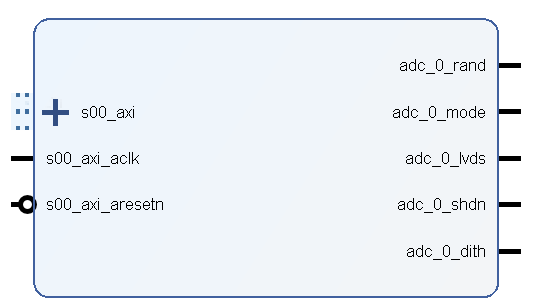
\includegraphics[width=\linewidth]{images/AXI_ADC_ctrl}
		\caption{Default-Single ADC}
	\end{subfigure}
	\begin{subfigure}[t]{0.4\linewidth}
		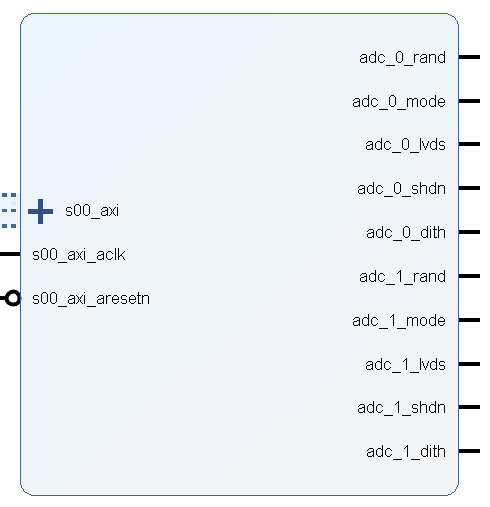
\includegraphics[width=\linewidth]{images/AXI_ADC_ctrl_extended}
		\caption{Outputs for Two ADCs}
	\end{subfigure}
	\caption{IP Integrator diagram of the AXI\textunderscore ADC\textunderscore ctrl}
\end{figure}
\subsection{Parameters}
Non-AXI related parameters:
\begin{description}
	\item[numChannels]Specifies the number of ADCs that will be controlled by the IP. The necessary output pins will become visible to accommodate the
		specified number.
\end{description}
\subsection{Pin Description}
Where \textit{x} is a place holder for the ADC number, from 0 to 31, that the pin is associated to.
\begin{description}
	\item[s00\textunderscore axi\textunderscore aclk]Active high AXI-Lite clock input
	\item[s00\textunderscore axi\textunderscore aresetn]Active low reset
	\item[adc\textunderscore \textit{x}\textunderscore mode]Active high GPIO output for `random' input of LTC2217
	\item[adc\textunderscore \textit{x}\textunderscore mode]Active high GPIO output for `mode' input of LTC2217
	\item[adc\textunderscore \textit{x}\textunderscore lvds]Active high GPIO output for `LVDS' input of LTC2217
	\item[adc\textunderscore \textit{x}\textunderscore shdn]Active high GPIO output for `shutdown' input of LTC2217
	\item[adc\textunderscore \textit{x}\textunderscore dith]Active high GPIO output for `dither' input of LTC2217
\end{description}
\subsection{AXI Register Mapping}
\begin{table}[H]
	\centering
	\caption{AXI\textunderscore ADC\textunderscore ctrl Register Map}
	\begin{tabular}{l|c|c|c|c|c|c}
		\toprule
		&\textbf{slv\textunderscore reg0}&\textbf{slv\textunderscore reg1}&\textbf{slv\textunderscore reg2}&
		 \textbf{slv\textunderscore reg3}&\textbf{slv\textunderscore reg4}&\textbf{slv\textunderscore reg5}\\
		\midrule
		bits 4-0&0&6&12&18&24&30\\
		\hline
		bits 9-5&1&7&13&19&25&31\\
		\hline
		bits 14-10&2&8&14&20&26&Unused\\
		\hline
		bits 19-15&3&9&15&21&27&Unused\\
		\hline
		bits 24-20&4&10&16&22&28&Unused\\
		\hline
		bits 29-25&5&11&17&23&29&Unused\\
		\hline
		bits 31-30&Unused&Unused&Unused&Unused&Unused&Unused\\
	\end{tabular}
\end{table}
The integers above represent ADC number that the five enclosed bits are mapped to. For example, the register bits in 15, spanning bits 19-15,
are mapped to the five outputs connected to the ADC 15, where each individual control line is mapped to the following bits:
\begin{table}[H]
	\centering \caption{Control Line Mapping for Each ADC}
	\begin{tabular}{c|c|c|c|c}
	\toprule
	\multicolumn{5}{c}{\textbf{adc\_{}\textit{x}\_{}outputs}}\\
	\midrule bit 4&bit 3&bit 2&bit 1&bit 0\\
	\hline adc\textunderscore \textit{x}\textunderscore rand&adc\textunderscore \textit{x}\textunderscore mode&adc\textunderscore \textit{x}
		\textunderscore lvds&adc\textunderscore \textit{x}\textunderscore shdn&adc\textunderscore \textit{x}\textunderscore dith\\
	\end{tabular}
\end{table}
\subsection{AXI Register Description}
Each bit in the registers are active high, and associated to the pin with the same name.
\subsection{Usage}
This IP requires a result pulse at boot up. After this, registers can be written with a logical one to turn on the associated pin. The state of the pins
will immediately change once the registers are updated from an AXI write.\hfill\break
As an example, if the user wants to turn on the adc\textunderscore 5\textunderscore mode pin, they should write a logical one into bit 28 of
slv\textunderscore reg0, since ADC five is located in bits 29-25 of slv\textunderscore reg0 and the mode bit is four bits over.\hfill\break
In addition, the registers can be read to query the state of the control pins.

\section{AXI\textunderscore DAC\textunderscore CTRL}
This IP is an AXI-Lite controlled IO unit, specifically for driving the clock and control IO lines of the MAX5885 digital to analog converter
\textit{DAC}.
Internally, a PRBS\textunderscore gen IP, and an OBUFDS primitive are instantiated to generate the random bit stream and differential sample clocks
required by the DAC. Unlike the AXI\textunderscore ADC\textunderscore ctrl, this IP is designed to be implemented within the DAC\textunderscore IF
\textunderscore core, but can be independently implemented if desired.
\subsection{Diagram}
\begin{figure}[H]
	\centering
	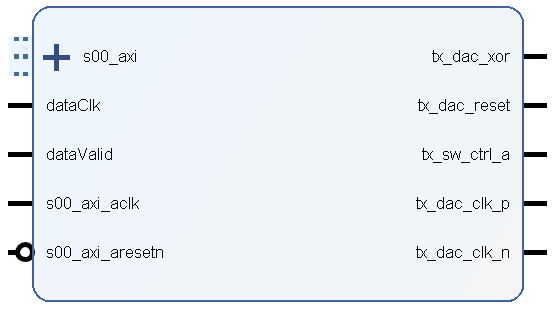
\includegraphics[width=0.42\linewidth]{images/AXI_DAC_CTRL}
	\caption{IP Integrator Diagram of the AXI\textunderscore DAC\textunderscore CTRL}
\end{figure}
\subsection{Parameters}
Non-AXI related parameters:
\begin{description}
	\item[randomGenBits]Number of bits used within internal random generator. Default is seven
	\item[reset\textunderscore tapAddr]Tap address for internal random number generator inserted in AXI register at reset. This will change the tap
		used when a reset is provided
	\item[reset\textunderscore xorOn]State of tx\textunderscore dac\textunderscore xor inserted in AXI register at reset. This will enable or disable the
		XOR feature when a reset is provided
\end{description}
\subsection{Pin Description}
\begin{description}
	\item[tx\_{}dac\_{}xor]XOR line on which a random bit stream will established when the XOR feature of this IP is enabled using the respective AXI
		register. The purpose of this line is to inform the DAC when the data has been randomly inverted so the DAC can re-invert it to its proper value.
		A logical one indicates that the data from the dac\textunderscore IF\textunderscore core has been inverted.
		For more information on the XOR function of the DAC, refer to the dac\textunderscore IF\textunderscore core.
	\item[tx\_{}dac\_{}reset]Active high reset pin for DAC
	\item[tx\_{}dac\_{}sw\_{}a]Active high control line that switches on the signal path
	\item[tx\_{}dac\_{}clk\_{}p]Positive differential sample clock output. This is in phase with the dataClk input and the transmit data
	\item[tx\_{}dac\_{}clk\_{}n]Negative differential sample clock output. This is directly out of phase with the dataClk input and the transmit data
	\item[dataClk]Single ended sample clock input
	\item[dataValid]Input that indicates when the dac\textunderscore IF\textunderscore core has valid transmit data. When this is low, the PRBS\_{}gen and
		DAC are reset, regardless of dedicated reset inputs
	\item[s00\textunderscore axi\textunderscore aclk]Active rising edge AXI-Lite clock
	\item[s00\textunderscore axi\textunderscore aresetn]Active low reset that resets the PRBS\textunderscore gen, the AXI-Lite registers, and the DAC
		with the tx\_{}dac\_{}sw\_{}
	\item[s00\textunderscore axi]AXI-Lite bus containing all necessary lines to meet the protocol
\end{description}
\subsection{AXI Register Mapping}
\begin{table}[H]
	\centering
	\caption{AXI-Lite Register Mapping for AXI\textunderscore DAC\textunderscore CTRL}
	\begin{tabular}{p{1.5cm}|p{1.5cm}|c|c|c|c}
		\toprule
		\textbf{Register Name}&\textbf{Address Offset}&\multicolumn{4}{c}{\textbf{Register Map (32bits per reg.)}}\\
		\midrule
		% slv_reg0
		\multirow{2}{*}{slv\textunderscore{}reg0}&\multirow{2}{*}{4'h0}&dynamic\textunderscore tapAddr&tx\_dac\_xor&tx\_dac\_reset&tx\_sw\_ctrl\_a\\
		\cline{3-6}
		&&bits 31-3&bit 2&bit 1&bit 0\\
		\hline
		% slv_reg1
		\multirow{2}{*}{slv\textunderscore{}reg1}&\multirow{2}{*}{4'h4}&\multicolumn{4}{c}{Unused}\\
		\cline{3-6}
		&&\multicolumn{4}{c}{bits 31-0}\\
		\hline
		% slv_reg2
		\multirow{2}{*}{slv\textunderscore{}reg2}&\multirow{2}{*}{4'h8}&\multicolumn{4}{c}{Unused}\\
		\cline{3-6}
		&&\multicolumn{4}{c}{bits 31-0}\\
		\hline
		% slv_reg3
		\multirow{2}{*}{slv\textunderscore{}reg3}&\multirow{2}{*}{4'hC}&\multicolumn{4}{c}{Unused}\\
		\cline{3-6}
		&&\multicolumn{4}{c}{bits 31-0}\\
		\bottomrule
	\end{tabular}
\end{table}
\subsection{AXI Register Description}
\begin{description}
	\item[dynamic\_tapAddr (w)]Output pin address of the random bit stream generator to connect to tx\_{}dac\_{}xor. This can be changed at runtime.
		Although 29 AXI register bits are allocated, in default operation, only the least significant four bits will modify the tap address and the rest
		will be ignored. If this IP is modified, the number of valid bits in this register becomes $log_2{randomGenBits}+1$, the same number of address
		bits the internal PRBS\_gen requires
	\item[tx\_dac\_xor (w)]Active high bit enabling or disabling the random bit stream generation
	\item[tx\_dac\_reset (w)]Active high reset for the DAC and PRBS\_gen. The AXI-Lite transceiver will not be reset upon assertion of this bit
	\item[tx\_dac\_sw\_ctrl\_a (w)]Active high bit that drives the tx\_{}dac\_{}sw\_{}a pin to the same state
\end{description}
\subsection{Usage}
\subsubsection{General}
This IP is designed to be implemented within the DAC\_IF\_core IP; nevertheless, it may also be used independently. It requires a reset pulse at boot up
and. Once complete, the I/O pins can be driven to the desired state by setting the appropriate AXI registers.
\subsubsection{Clocking}
A single-ended sample clock is supplied to the AXI\textunderscore DAC\textunderscore CTRL where it is converted to 3.3 V differential CMOS lines for the
MAX5885. The CLKP and CLKN input clock pins on the MAX5885 are LVPECL (\textit{Low Voltage Positive Emitter Coupled Logic}), but the 7-Series FPGAs don't
contain LVPECL logic. Luckily, these clock inputs are rated for 3.3 V and are AC coupled on the Jay-1 TRX board, allowing them to be driven with CMOS
signals. In order to use the 3.3 V CMOS clock signals provided by this IP, VCLK on the MAX5885 needs to be 3.3 V. 

\section{shift\textunderscore register}
This IP is a completely configurable shift register, including a configurable size, configurable control pins, and configurable modes of operation. It
should be noted that registers are implemented in FPGA fabric, not in dedicated BRAM. All of the following modes are supported:
\begin{itemize}
	\item PIPO - \textit{Parallel In, Parallel Out}
	\item PISO - \textit{Parallel In, Serial Out}
	\item SIPO - \textit{Serial In, Parallel Out}
	\item SISO - \textit{Serial In, Serial Out} 
\end{itemize}
\subsection{Diagram}
The default configuration, shown below, enables all available control pins in a PIPO configuration with output latches enabled.
When the input or output mode is set to serial, the input/output channel will scale to a single bit wide.
\begin{figure}[H]
	\centering
	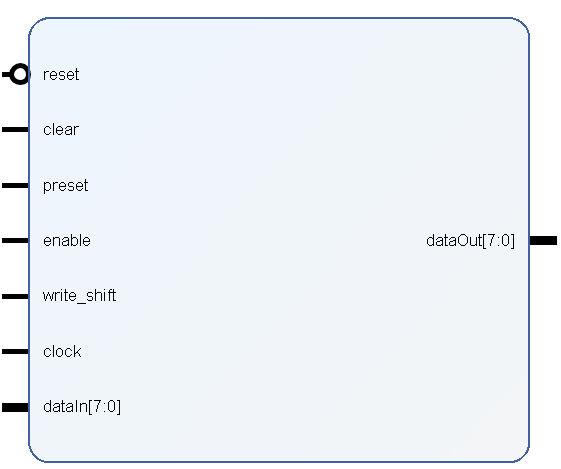
\includegraphics[width=0.4\linewidth]{images/shift_register}
	\caption{IP Integrator Diagram of the shift\textunderscore register}
\end{figure}
\subsection{Parameters}
\begin{description}
	\item[size]Number of bits/flip-flops to internally instantiate. Outputs and inputs scale accordingly
	\item[resetValue]Decimal representation of the bit array desired at the output of the internal flip-flops. Default is zero
	\item[parallel\textunderscore input\textunderscore en]Single bit which enables or disables the parallel input feature. When disabled, with a logical
		zero, the input mode will become serial. The default is 1'b1 (parallel input enabled)
	\item[parallel\textunderscore output\textunderscore en]Single bit which enables or disables the parallel output feature. When disabled, with a logical
		zero, the output mode will become serial. The default is 1'b1 (parallel output enabled)
	\item[output\textunderscore latch\textunderscore en]Single bit which enables or disables the output latch feature. When disabled, with a logical zero,
		no output latches are instantiated and the latch\textunderscore pin is removed. The default is 1'b1
	\item[preset\textunderscore en]Enables the synchronous preset input pin
	\item[clear\textunderscore en]Enables the synchronous clear input pin
	\item[enable\textunderscore en]Enables the synchronous enable input pin
\end{description}
\subsection{Pin Description}
\begin{description}
	\item[reset]Active low reset input, driving output of all internal flip-flops to the value specified with resetValue. This pin has the highest control
		pin priority.
	\item[clear]Active low clear input, driving output of all internal flip-flops to zero. This pin has the second highest control pin priority.
	\item[preset]Active low preset input, driving output of all internal flip-flops to one. This pin has the third highest control pin priority.
	\item[enable]Active low enable input, enabling all internal flip-flops to change state. This pin has the lowest control pin priority.
	\item[latch\textunderscore control]Active rising edge input that latches the flip-flop states to the output pins.
	\item[write\textunderscore shift]Input determining whether the shift\textunderscore register will accept a write from the parallel input wires
		(logical zero), or will shift the data currently stored (logical one) on the following positive clock edge. This pin is only enabled when parallel
		\textunderscore input\textunderscore en is set to 1'b1
	\item[clock]Active rising edge clock for loading and shifting data
	\item[dataIn]Channel for input data. Adjusts size and connection based on the parameters specified
	\item[dataOut]Channel for output data. Adjusts size and connection based on the parameters specified
\end{description}
\subsection{Operation}
A reset pulse should be delivered at boot up to initialize the flip-flop states to the value specified with the resetValue parameter. In parallel input
mode, the write\textunderscore  shift input selects whether to write the data on the input lines to the flip flops or shift the data currently there, if
permitted by the control lines. Serial input mode will connect the dataIn channel to the first flip-flop's input, and serial output mode will connect the
dataOut channel to the last flip-flop's non inverted output.\hfill\break
This device supports configurable output latches, which are enabled by setting
output\textunderscore latch\textunderscore en to 1'b1. When enabled, a logic high on the latch\textunderscore control input will latch whatever data is
on the output(s) to the output pins. These latches are not affected by the control inputs, and will simply output the last latched value until the
latch\textunderscore control becomes high.

\section{PRBS\textunderscore gen}
The PRBS\textunderscore gen stands for \textit{Pseudo Random Bit Sequence Generator}, and is a configurable source for random values. Internally, it
contains a parallel output shift\textunderscore register, used to create \textit{Linear Feedback Shift Register} for random number generation. Exclusive
NOR gates are used in the feedback path and are automatically instantiated and connected based on the parameters to maximize the sequence length. This IP
supports variable seeds, single and parallel outputs, dynamic tap addressing, and variable size. Available bit lengths are 2-786, 1024, 2048, and 4096.
When the output is serial, the \textit{tap} refers to which shift register output the output pin is connected to.
\subsection{Diagram}
Both diagrams are shown with a bit length of four.
\begin{figure}[H]
	\centering
	\begin{subfigure}[t]{0.45\linewidth}
		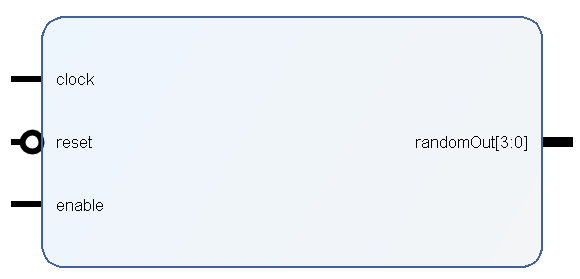
\includegraphics[width=\linewidth]{images/PRBS_gen_default}
		\caption{Default Configuration}
	\end{subfigure}
	\begin{subfigure}[t]{0.35\linewidth}
		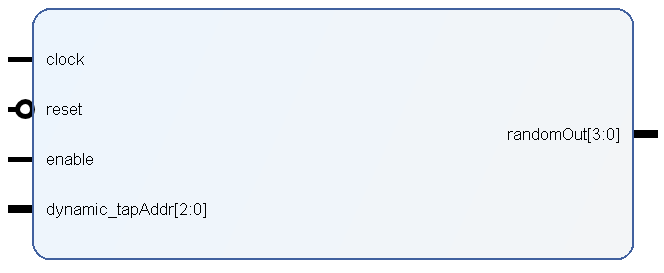
\includegraphics[width=\linewidth]{images/PRBS_gen_dynamic}
		\caption{Dynamically Tapped}
	\end{subfigure}
	\caption{IP Integrator Diagram of the PRBS\textunderscore gen}
\end{figure}
\subsection{Parameters}
\begin{description}
	\item[numBits]Number of bits/flip-flops used in \textit{LFSR}
	\item[parallel\textunderscore out\textunderscore en]Single bit to enable or disable parallel output. When disabled with a logical zero, the output
		becomes serial, tapped either statically or dynamically
	\item[seed]Decimal value of the seed for random number generation. This is the value of the shift register output lines at reset
	\item[enable\textunderscore en]Single bit enabling the enable input terminal on the device
	\item[static\textunderscore tapAddr]Zero indexed address of the shift register output to which the serial output shall be connected in serial output
		mode. This value is zero by default, and only applies if dynamic\textunderscore tap\textunderscore en is inactive
	\item[dynamic\textunderscore tap\textunderscore en]Single bit enabling or disabling the dynamic tap addressing feature. The dynamic\textunderscore
		tapAddr input pins will be visible when this parameter is set to 1'b1
\end{description}
\subsection{Pin Description}
\begin{description}
	\item[clock]Rising edge active clock used to generate a new random value
	\item[reset]Active low synchronous reset pin
	\item[enable]Active high synchronous enable pin. While inactive, this pin will prevent the device from proceeding to the following random number.
		Clock signals while disabled will be ignored
	\item[randomOut]Output channel for random values. Scales based on the parallel\textunderscore out\textunderscore en parameter
	\item[dynamic\textunderscore tapAddr]Input channel for dynamic tap address which is only visible when the dynamic tap is enabled and is used to select
		the desired tap between the serial output and shift register output. The width of this channel is automatically calculated as $log_2(numBits)+1$
\end{description}
\subsection{Usage}
This IP requires a reset pulse to be delivered at boot up to initialize the shift register output lines to the seed value. After this, with the enable pin
high, a new random value will be generated at every rising positive edge. When using serial output, the output channel is connected to a single shift
register output pin, which is selectable statically or dynamically using the appropriate parameters and addressing.

\section{channel\textunderscore delay}
This IP is an extensible wrapper around the IDELAYE2 primitive, allowing multiple to be instantiated within a single IP, thereby creating a channel. In
7-series FPGAs, each I/O block contains an IDELAYE2 element, and each element can only access the input within its I/O block. As a result, each line
within the channel\textunderscore delay IP has an independent delay element. Nevertheless, the channel\textunderscore delay IP only supports a single,
fixed tap value for all delay elements. This design creates the perception of a single delay element which delays all lines within a channel to the same
degree. 
Further information regarding the internal IDELAYE2 primitive from Xilinx can be found in the \textit{UG953} reference guide.
\subsection{Diagram}
\begin{figure}[h!]
	\label{fig:channel_delay}
	\centering
	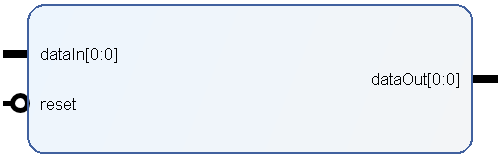
\includegraphics[width=0.6\linewidth]{images/channel_delay}
	\caption{IP Integrator Diagram of the channel\textunderscore delay}
\end{figure}
\subsection{Parameters}
\begin{description}
	\item[numElements]Width of delay channel
	\item[refClkFreq]The frequency in MHz of the reference clock, provided through an IDELAYCTRL module. Available value are 190-210 MHz and 290-310 MHz
		for the 7-Series FPGAs
	\item[highPerformance\textunderscore delay]Enables or disables high performance mode of the IDELAYE2 in exchange for power savings. Available options
		are ``TRUE" and ``FALSE"
	\item[delayVal]Selectable tap value which selects the delay imposed upon the signal, equal to $1/(64\times refClkFreq)\mu{}S$, where refClkFreq is
		in MHz
	\item[signalType]Describes the signal type for the internal IDELAYE2. Available values are ``CLOCK" and ``DATA", and the default value is ``DATA"
\end{description}
\subsection{Pin Description}
\begin{description}
	\item[dataIn]Input channel
	\item[dataOut]Output channel
	\item[reset]Active low reset
\end{description}
\subsection{Usage}
As this IP includes an IDELAYE2, it requires an IDELAYCTRL device to be instantiated in the same design in order to maintain calibration. Although there
is not a physical wire routed between the two, there is an internal bus designated for the reference clock signals in the FPGA, and once both are
instantiated, they will be placed on this bus upon implementation.

\section{dac\textunderscore IF\textunderscore core}
This IP is specifically designed to interface and control the MAX5885 digital to analog controller (\textit{DAC}) within the transmit path of the Jay-1
ionosonde. It acts as an AXI-Stream slave, receiving 16-bit samples and directing them to the DAC over 16 parallel CMOS 3.3 V lines. In addition, this IP
provides an AXI-Lite interface for configuration and settings during runtime.\hfill\break
The output signal passes through a delay\_FIFO for delay tuning, and can be inverted for the XOR feature of the MAX5885. A channel\_delay element is
contained in the output path for the DAC sample clock, allowing phase tuning of the sample clock to meet the sample data.\hfill\break
In addition, a power\_meter is housed within this IP, and directly reads the transmit power from the AXI-Stream input port. This power meter, along with
the delay\_FIFO, and AXI\_DAC\_CTRL can all be communicated with through a single AXI-Lite interface with the help of a contained crossbar.\hfill\break
Internally, this IP contains the logic to prevent data corruption from enablement or reset while the IP is busy, and logic to meet reset requirements of
contained IP.\hfill\break
For further information on the MAX5885, please refer to its data sheet located below.
\captionsetup[table]{list=no}   % exclude this from table list
\subsection{Contained IP}
\begin{table}[H]
	\centering
	\caption{Contained IP Within adc\textunderscore IF\textunderscore core}
	\begin{tabular}{p{6cm}|p{6cm}}
		\multicolumn{1}{c|}{\textbf{Custom IP}}&\multicolumn{1}{|c}{\textbf{Xilinx IP}}\\
		\toprule		
		\begin{itemize}
	 		\item channel\_delay
			\item AXI\_DAC\_CTRL
			\item power\textunderscore meter
			\item delay\textunderscore FIFO
			\item IDELAYBUFDS
		\end{itemize}
		&
		\begin{itemize}
			\item axi\textunderscore crossbar
			\item util\textunderscore reduced\textunderscore logic
			\item util\textunderscore vector\textunderscore logic
			\item xlconcat
			\item xlslice
		\end{itemize}\\
	\end{tabular}
\end{table}
\captionsetup[table]{list=yes}   % include following tables
\subsection{Diagrams}
\begin{figure}[H]
	\centering
	\begin{subfigure}[b]{\linewidth}
		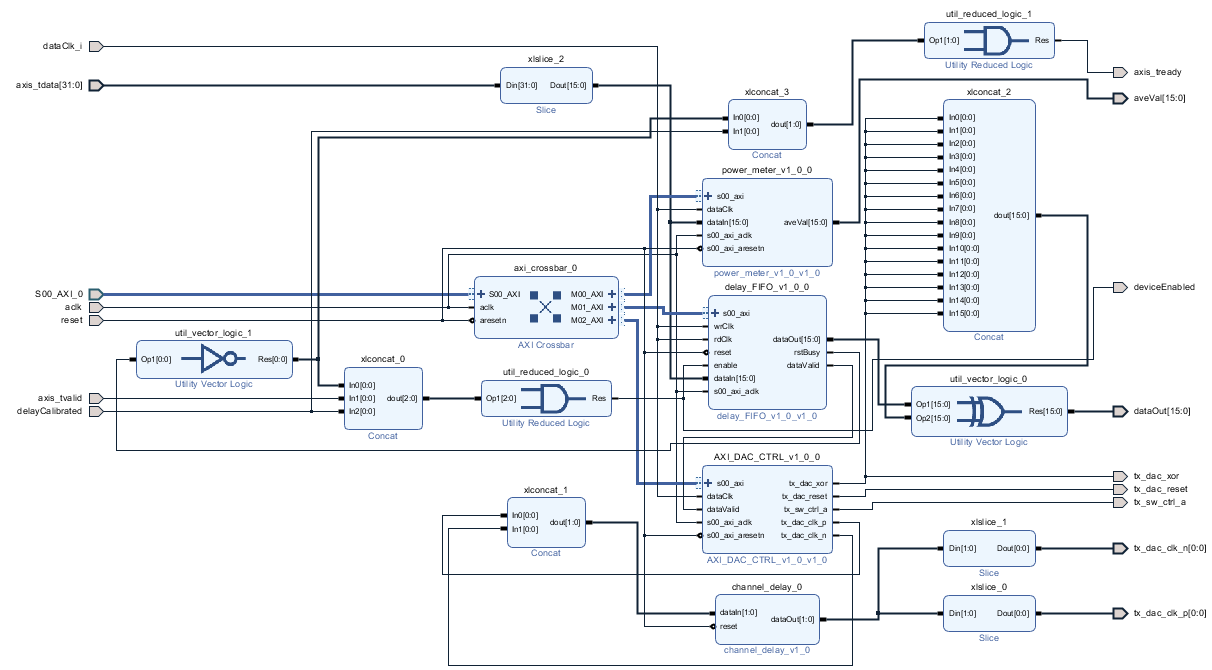
\includegraphics[width=\linewidth]{images/dac_IF_core_internal}
		\caption{Internal Diagram}
	\end{subfigure}
	\begin{subfigure}[b]{0.4\linewidth}
		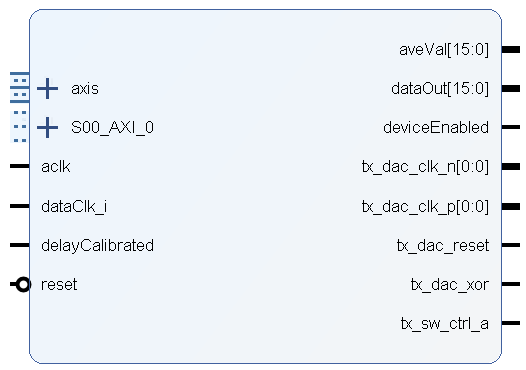
\includegraphics[width=\linewidth]{images/dac_IF_core}
		\caption{dac\textunderscore IF\textunderscore core Package}
	\end{subfigure}
	\caption{IP Integrator Diagrams of the dac\textunderscore IF\textunderscore core}
\end{figure}
\subsection{Parameters}
Since this IP is very specific to its application, it does not contain any global parameters. All internal IP is pre-configured to meet the application
requirements. Sadly, the IP flow does not support passing global parameters to internal IP, preventing externalizing composing IP's parameters. The 
delayVal parameter of the channel\_delay suffers most from this, as it may need modification to match the sample data phase. If one would like to alter
these default parameters, they can do so by modifying the design in the IP Integrator and re-packaging.
\subsubsection{Internal IP Default Parameters}
Every IP has default parameters, most of which are obvious or are described by the IP operation. The important parameters are listed in the following
figures.
\begin{figure}[H]
	\centering
	\begin{subfigure}[t]{0.4\linewidth}
		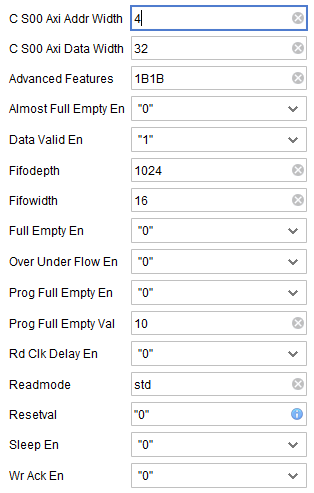
\includegraphics[width=\linewidth]{images/default_dac_param_delay_FIFO}
		\caption{delay\textunderscore FIFO}
	\end{subfigure}
	\begin{subfigure}[t]{0.4\linewidth}
		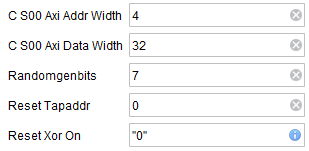
\includegraphics[width=\linewidth]{images/default_dac_param_dac_ctrl}
		\caption{AXI\_DAC\_CTRL}
	\end{subfigure}
	\begin{subfigure}[t]{0.4\linewidth}
		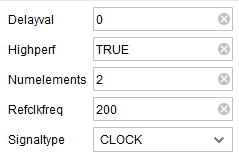
\includegraphics[width=\linewidth]{images/default_dac_param_channel_delay}
		\caption{channel\textunderscore delay}
	\end{subfigure}
	\begin{subfigure}[t]{0.4\linewidth}
		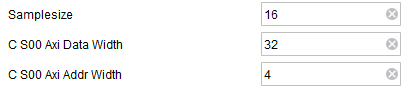
\includegraphics[width=\linewidth]{images/default_dac_param_power_meter}
		\caption{power\textunderscore meter}
	\end{subfigure}
	\caption{Default Parameters of the dac\textunderscore IF\textunderscore core's Internal IP} 
	\label{fig:dacIFparams}
\end{figure}
\subsection{Pin Description}
\begin{description}
	\item[aclk]AXI-Lite active rising edge clock
	\item[reset]Active low reset for all logic, including AXI-Lite interface
	\item[dataClk\_i]Single-ended, active rising edge sample. Essentially the AXI-Stream clock from the AXI-Stream master which is in phase with the
		input data. Writes and reads data to and from the dac\_IF\_core,
	\item[delayCalibrated]Flag from IDELAYCTRL module that must be instantiated within the same design as this IP. Informs the dac\textunderscore IF
		\textunderscore core that the delay filter is stable/calibrated. This IP is internally prohibited from reading from the AXI-Stream
		interface or writing to the DAC through the FIFO while this is low.
	\item[aveVal]16-bit, single-ended output channel from the internal power\textunderscore meter, relaying the average power for other hardware devices
	\item[dataOut]16-bit, single-ended output channel that sends the transmit data to the DAC. This data may be inverted for the XOR functionality, and
		delayed for phase tuning.
	\item[tx\_dac\_clk\_n]Negative CMOS output terminal with the data clock. This signal may be delayed for phase tuning with the internal channel\_delay
		but will always be $180^{\circ}$ out of phase with tx\_dac\_clk\_p
	\item[tx\_dac\_clk\_p]Positive CMOS output terminal with the data clock. This signal may be delayed for phase tuning with the internal channel\_delay
		but will always be $180^{\circ}$ out of  phase with tx\_dac\_clk\_n
	\item[tx\_dac\_reset]Active high reset pin for the DAC
	\item[tx\_dac\_xor]Active high output which, when the feature is activated, contains a random bit stream for XOR inversion
	\item[tx\_sw\_ctrl\_a]Active high output which activates the transmit path switch
	\item[deviceEnabled]Active high output flag which indicates the internal FIFO is enabled; the IP is able to receive data. Specifically, this
		indicates:
		\begin{enumerate}
			\item delayCalibrated is high 
			\item AXI-Stream interface contains valid data, indicated by a logic one on the valid pin
			\item the FIFO is not within its reset procedure
			\item active low reset line is deactivated
		\end{enumerate}
	\item[axis]AXI-Stream interface. Contains necessary lines to match protocol. As these lines are simple enough to be implemented in a design with
		discrete logic, their purposes are listed below:\hfill
		\begin{description}
			\item[$\bullet$ axis\textunderscore tvalid]Indicates to the slave that valid data is available
			\item[$\bullet$ axis\textunderscore tready]Indicates to the master that the slave is ready for data
			\item[$\bullet$ axis\textunderscore tdata]32-bit data channel
		\end{description}
		A master must implement the valid and data signals and read the ready line.
	\item[S00\textunderscore AXI\textunderscore 0]AXI-Lite bus containing all necessary lines for the protocol
\end{description}
\subsection{AXI Interface Mapping}
Both the AXI-Stream data channel mapping and the AXI-Lite address mapping are included in this section. For a detailed mapping of each register, please 
refer to the respective IP description above.
\subsubsection{AXI-Stream Interface}
\begin{table}[H]
	\centering
	\caption{Data Channel Mapping - axis\textunderscore tdata}
	\begin{tabular}{|c|c|}
		\toprule
		\multicolumn{2}{|c|}{\textbf{Channel: bits 31 - 0}}\\
		\midrule
		Unused&dataOut\\
		\hline
		bits 31 - 16&bits 15-0\\	
		\hline
		\multicolumn{1}{|c|}{left unconnected}&\multicolumn{1}{c|}{data input containing transmit samples}\\
		\bottomrule
	\end{tabular}
\end{table}
\subsubsection{AXI-Lite Address Mapping}
The following AXI-Lite devices are connected through a crossbar, allowing them to be accessible through the single S00\textunderscore AXI\textunderscore 0
interface.
\begin{table}[H]
	\centering
	\caption{dac\textunderscore IF\textunderscore core AXI-Lite Address Mapping}
	\begin{tabular}{c|c|c|c|c}
		\textbf{Internal IP}&\textbf{Address Bits}&\textbf{Offset Address}&\textbf{Range}&\textbf{High Address}\\
		\midrule
		AXI\_DAC\_CTRL&32&0x44A00000&4K&0x44A00FFF\\
		delay\textunderscore FIFO&32&0x44A10000&4K&0x44A10FFF\\
		power\textunderscore meter&32&0x44A20000&4K&0x44A20FFF\\
	\end{tabular}
\end{table}
\subsection{Usage}
\subsubsection{General}
This IP requires a reset pulse to be delivered at start up. Once the device is ready for operation, the deviceEnabled line will go high, allowing the 
internal FIFO to begin reading and writing data. Most harmful events are prevented from existing in this IP, but is often done by ignoring input data and
clocks while the device is in a busy state. So long as important data is not written while the deviceEnabled line is low, this should not be an issue.
Once deviceEnabled becomes high, data will be read by this IP, and, after the appropriate delay has passed, written to the DAC. In
addition, the AXI\_DAC\_CTRL, delay\textunderscore FIFO, and power\textunderscore meter will become accessible over AXI-Lite, where each can be written to
and read from. Although they are not physically prevented, these AXI-Lite connected IP should not be communicated with while in a reset state.
\hfill\break
In order to modify the internal IP's parameters, most notably the delayVal of the channel\_delay, one must edit the dac\textunderscore IF\textunderscore
core block design and re-package, since the IP Integrator design flow does not support externalizing parameters.
\subsubsection{XOR Data Inversion}
In order to decorrelate the input bit transitions from the DAC output, the MAX5885 supports XOR inversion. When the data signal is randomly inverted with
XOR gates, the EMI produced will contain a wide frequency content of lower amplitude. To support this feature, bank of XOR gates is located on the MAX5885
data input and the dac\_IF\_core data output. When enabled over the AXI-Lite interface, the AXI\_DAC\_CTRL will generate a random bit stream which gets
delivered to the output inversion bank, and to the MAX5885, over tx\_dac\_xor, so the data can be re-inverted.

\section{VGA\_SW\_IF}
This IP is an interface specifically built for the LMH6517 variable gain amplifier \textit{VGA} and RF switch located on the receiver path of the Jay-1
ionosonde. It receives input from the gain compensation block, for long term gain bias, and an input from the automated gain control algorithm
(\textit{AGC}), which determines the optimal gain for the ADC based on the received signal power level. Both inputs to this IP are in tenths of a dB, or
cB. This IP contains an internal state machine that provides the LMH6517 with the pulse interface it requires to modify the VGA gain based the two inputs,
and reset the device. Furthermore, this IP contains a AXI-Lite interface for configuration and software control, and a timing clock to meet the strict
pulse timing requirements of the LMH6517's pulse interface. For more information on this VGA, please refer to \textit{SNOSB19K}.
\subsection{LMH6517 Block Diagram}
\begin{figure}[H]
	\centering
	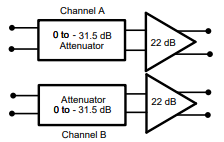
\includegraphics[width=0.35\linewidth]{images/vga_blockDiagram}
	\caption{Block Diagram of LMH6517 VGA}
\end{figure}
\subsection{Diagram}
The default configuration is shown below, which has all pins enabled.
\begin{figure}[H]
	\centering
	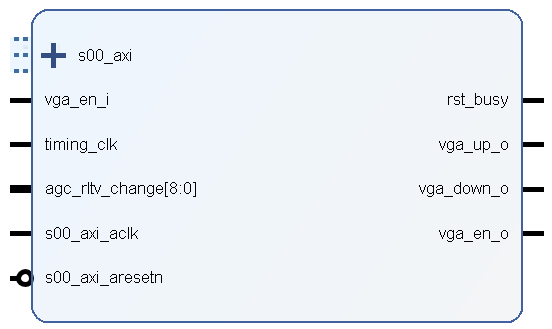
\includegraphics[width=0.4\linewidth]{images/vga_sw_if}
	\caption{IP Integrator Diagram for the VGA\_SW\_IF}
\end{figure}
\subsection{Parameters}
Non-AXI related parameters:
\begin{description}
	\item[max\_gain]Maximum gain possible by the VGA in tenths of a dB. Default value is 220 and this parameter must contain an integral multiple of
		five tenths of a dB
	\item[min\_gain]Minimum gain possible by the VGA in tenths of a dB. Default value is -95 and this parameter must contain an integral multiple of
		five tenths of a dB
	\item[vgaEnable\_en]Single active high bit that enables or disables the hardware vgaEnable pin on the IP
	\item[nominal\_gain]VGA gain desired at reset in tenths of a dB. This parameter must contain an integral multiple of
		five tenths of a dB and must be within max\_gain and min\_gain. The default value is 160 
\end{description}
\subsection{Pin Description}
\begin{description}
	\item[vga\_en\_i]Active high input enable pin for VGA. Either a logic one on this input or the enable AXI register will cause the device to be enabled
		, so long as the disable pin is low, which has the highest priority. This hardware pin can removed with the vgaEnable\_en parameter
	\item[timing\_clk]Clock used to ensure timing requirements for VGA pulses are met. This clock should have a period equal to the hold time of the pulse
		lines - 20 ns in this case. As such, in the current design this should be 50 MHz
	\item[agc\_rltv\_change]Desired relative gain change from the AGC, with reference to nominal\_gain, in tenths of a dB. These bits should be formatted
		in two's complement and must contain a integral multiple of five tenths of a dB
	\item[rst\_busy]Active high output flag indicating that the device is within its reset sequence. This should control the RF input switch
	\item[vga\_up\_o]Active low \textit{up} line for pulse interface to VGA. An independent low pulse of this line will raise the VGA gain by 0.5dB, if
		permitted
	\item[vga\_down\_o]Active low \textit{down} line for pulse interface to VGA. An independent low pulse of this line will reduce the VGA gain by 0.5dB,
		if permitted
	\item[vga\_en\_o]Active high output enable for VGA
	\item[s00\_axi\_aresetn]Active low reset for VGA and AXI-Lite. A low pulse of this pin or the reset AXI bit will cause the device to enter the reset
		sequence
	\item[s00\_axi]AXI-Lite bus that contains all signals for the protocol
\end{description}
\subsection{AXI Register Mapping}
\begin{table}[H]
	\centering
	\caption{VGA\_SW\_IF Register Map}
	\begin{tabular}{|l|c|c|c|c|}
		\toprule
		&\textbf{slv\textunderscore reg0}&\textbf{slv\textunderscore reg1}&\textbf{slv\textunderscore reg2}&
		 \textbf{slv\textunderscore reg3}\\
		\midrule
		bits 0-8&comp\_rltv\_change&current\_rltv\_output&\multirow{10}{*}{Unused}&\multirow{10}{*}{Unused}\\
		\cline{1-3}
		bit 9&reset&\multirow{4}{*}{current\_rltv\_agc\_val}&&\\
		\cline{1-2}
		bit 10&enable&&&\\
		\cline{1-2}
		bit 11&disable&&&\\
		\cline{1-2}
		bits 12-17&\multirow{6}{*}{Unused}&&&\\
		\cline{1-1}\cline{3-3}
		bits 18-26&&nominal\_gain&&\\	
		\cline{1-1}\cline{3-3}
		bit 27&&rst\_busy&&\\
		\cline{1-1}\cline{3-3}
		bit 28&&underflow&&\\
		\cline{1-1}\cline{3-3}
		bit 29&&overflow&&\\
		\cline{1-1}\cline{3-3}
		bits 30-31&&Unused&&\\
		\bottomrule
	\end{tabular}
\end{table}
\subsection{AXI Register Description}
\begin{description}
	\item[disable (w)]Regardless of the enable AXI bit's or enable input pin's state, a logical one on this pin will disable the device
	\item[enable (w)]Active high enable bit. This bit, or a logical one on the enable input pin, will enable device, so long as the disable bit is
		inactive. At reset, this bit is internally driven high so this IP can be used without having to perform an AXI write
	\item[reset (w)]Active low reset bit. A logic zero on this bit or on the s00\_axi\_aresetn pin will cause this IP to enter its reset sequence and
		will reset the AXI-Lite interface. At reset, this bit is driven high so the device can be used without having to perform an AXI write
	\item[comp\_rltv\_change (w)]Compensation Relative Change: these bits receive the desired relative change in gain from the gain compensation in tenths
		of a dB. These bits should be formatted in two's complement and must contain an integral multiple of five tenths of a dB.
	\item[overflow (r)]Active high flag indicating an overflow condition has occurred
	\item[underflow (r)]Active high flag indicating an underflow condition has occurred
	\item[rst\_busy (r)]Active high flag indicating when the IP is within its reset sequence. Also indicates the state of the RF input switch
	\item[nominal\_gain (r)]Nominal gain parameter set upon compilation. Allows software to read value if required. This is formatted as a two's
		complement number in tenths of a dB
	\item[current\_rltv\_val (r)]Current relative difference between VGA\_gain and nominal\_gain in tenths of a dB. This will update as each pulse is
		delivered and is formatted in two's complement
	\item[current\_rltv\_agc\_val (r)]Current relative difference between agc\_rltv\_change and nominal\_gain in tenths of a dB. This will update as the
		AGC value changes and is formatted in two's complement
\end{description}
\subsection{Usage and Operation}
\subsubsection{General}
This IP requires a reset pulse to be delivered at boot up. After the rstBusy line goes low, the reset sequence has completed, and the VGA gain will be 
modified in accordance with the two relative inputs. However, at any instance that the vga\_en\_i line goes low, the VGA\_SW\_IF will stop delivering
pulses to the VGA and the vga\_en\_o will be driven low.\hfill\break
Each individual VGA channel requires an independent VGA\_SW\_IF. The LMH6517 contains two channels, and as such, if both are operational, two VGA\_SW\_IFs
are required.\hfill\break
In addition, the agc\_rltv\_change and comp\_rltc\_change can be overwritten at any rate to any value. This IP will simply direct the VGA gain to the
latest value, even if it has yet to reach the previous value.
\subsubsection{Reset Sequence}
Inherently, the LMH6517 sets its gain to the maximum possible value of 22.0 dB upon receiving a reset. This could be destructive to the ADC or other
receiver components, as they may become overloaded at reset. In order to avoid this, the VGA\_SW\_IF generates a reset sequence, where it will turn off
the RF input switch, reset the VGA, configure the gain down to the nominal value, and then turn on the RF input switch.
\subsection{Pulsed Interface} 
A pulsed interface is employed by this IP to modulate the gain on the LMH6517, which it natively supports. This consists of an up and down line, each of 
which are active low. When either line goes low for 20 ns, with a minimum setup time of 20 ns, the VGA gain moves in the associated direction by 0.5dB.
As a result, the slew rate for gain variation is very slow - 0.5dB/40ns.\hfill\break
The VGA\_SW\_IF ensures that this timing is met with the help of the timing\_clk.
\begin{figure}[H]
	\centering
	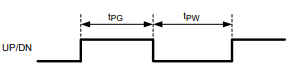
\includegraphics[width=0.4\linewidth]{images/vga_pulse_timing}
	\caption{Pulse Timing Requirement}
\end{figure}
\subsubsection{Overflow and Underflow Detection}
The values in comp\_rltv\_change and agc\_rltv\_change get internally summed, where the result becomes the desired deviation from the nominal gain that
the VGA will be driven to. This IP detects both over and underflow conditions when this sum produces an arithmetic binary over or underflow, and when the
sum exceeds the bounds of $max\_gain-nominal\_gain$ and $min\_gain-nominal\_gain$. At any of these incidents, the gain will be driven to min\_gain and the
associated flags will be set until an acceptable value is provided.

%Don't want any in text citations within the IP Catalog, so the links and references are just written manually instead of using bibtex
\newpage
\section{References and Links}
\paragraph{LT0108}Linear Technology. (n.d.). 16-Bit, 105Msps Low Noise ADC. Retrieved August 15, 2019, 
from https://www.analog.com/media/en/technical-documentation/data-sheets/2217f.pdf
\paragraph{DAC}Maxim Integrated. (2003, December). 3.3V, 16-Bit, 200Msps High Dynamic Performance DAC with CMOS Inputs. Retrieved August 15, 2019,
from https://datasheets.maximintegrated.com/en/ds/MAX5885.pdf
\paragraph{PRBS} Pini, A. (2018, March 22). Use Readily Available Components to Generate Pseudo-Random Binary Sequences and White Noise. Retrieved August 
15, 2019,from https://www.digikey.ca/en/articles/techzone/2018/mar/use-readily-available-components-generate-binary-sequences-white-noise  
\paragraph{SNOSB19}Texas Instruments.(2013, March). Low Power, Low Noise, IF and Baseband, Dual 16 bit ADC Driver With Digitally Controlled Gain.
Retrieved August 15, 2019, from https://www.ti.com/lit/ds/symlink/lmh6517.pdf 
\paragraph{UG953}Xilinx. (2018, June 6). Vivado Design Suite 7 Series FPGA and Zynq-7000 SoC Libraries Guide. Retrieved August 15, 2019,
from https://www.xilinx.com/support/documentation/sw\_manuals/xilinx2018\_2/ug953-vivado-7series-libraries.pdf
\paragraph{DS182}Xilinx. (2019, June 28). Kintex-7 FPGAs Data Sheet: DC and AC Switching Characteristics. Retrieved August 15, 2019, from\break
https://www.xilinx.com/support/documentation/data\_sheets/ds182\break\_Kintex\_7\_Data\_Sheet.pdf
\end{document}
